% ============================================================
%  Minimum-Container Packing of a Non-Convex Polygon
%  via Simulated Annealing and Bracketing-Bisection Search
%
%  Joel Solis, University of Arizona
%  Applied Mathematics and Numerical Methods
% ============================================================

\documentclass[10pt,twocolumn]{article}

% ---- Typography -------------------------------------------------
\usepackage{lmodern}
\usepackage[T1]{fontenc}
\usepackage{microtype}
\linespread{0.96}

% ---- Page geometry ---------------------------------------------
\usepackage[
  left=1.65cm, right=1.65cm,
  top=2.6cm,   bottom=2.4cm,
  headheight=13pt,
  headsep=10pt
]{geometry}
\setlength{\columnsep}{18pt}
\setlength{\columnseprule}{0.35pt}   % thin column divider

% ---- Running headers -------------------------------------------
\usepackage{fancyhdr}
\pagestyle{fancy}
\fancyhf{}
\fancyhead[LO]{\small\itshape Polygon Packing via Simulated Annealing and Bisection}
\fancyhead[RE]{\small\itshape J. Solis}
\fancyhead[RO,LE]{\small\thepage}
\renewcommand{\headrulewidth}{0.4pt}

\fancypagestyle{firstpage}{%
  \fancyhf{}
  \fancyhead[L]{\small\itshape
    Applied Mathematics and Numerical Methods --- University of Arizona, 2026}
  \fancyhead[R]{\small\thepage}
  \renewcommand{\headrulewidth}{0.4pt}%
}

% ---- Section headings ------------------------------------------
\usepackage{titlesec}
\titleformat{\section}[block]
  {\normalfont\bfseries\small\centering}
  {\thesection.}{0.4em}{\MakeUppercase}
\titleformat{\subsection}[block]
  {\normalfont\itshape\small}
  {\thesubsection.}{0.4em}{}
\titlespacing*{\section}   {0pt}{7pt plus 2pt minus 1pt}{3pt plus 1pt}
\titlespacing*{\subsection}{0pt}{5pt plus 1pt minus 1pt}{2pt plus 1pt}

% ---- Math, floats, tables --------------------------------------
\usepackage{amsmath,amssymb}
\usepackage{graphicx}
\usepackage{booktabs,array}
\usepackage[hidelinks]{hyperref}
\usepackage[
  font=small,
  labelfont=bf,
  labelsep=period,
  justification=justified
]{caption}
\setlength{\abovecaptionskip}{4pt}
\setlength{\belowcaptionskip}{0pt}
\usepackage{enumitem}
\setlist{noitemsep,topsep=1pt,leftmargin=*}

% ---- Abstract environment --------------------------------------
\usepackage{abstract}
\renewcommand{\abstractname}{}
\renewcommand{\absnamepos}{empty}
\setlength{\absleftindent}{0pt}
\setlength{\absrightindent}{0pt}

% ---- Spacing ---------------------------------------------------
\setlength{\parskip}{2pt}
\setlength{\parindent}{11pt}
\setlength{\abovedisplayskip}{5pt plus 2pt minus 2pt}
\setlength{\belowdisplayskip}{5pt plus 2pt minus 2pt}

% ================================================================
% Title block
% ================================================================
\title{%
  \Large\bfseries
  Non-Convex Polygon Packing via Simulated Annealing%
}

\author{%
  Joel Solis%
  \thanks{Department of Mathematics, University of Arizona.
          \texttt{jsolis@math.arizona.edu}.
          This work was supported by allocation math589 on the
          University of Arizona HPC cluster.}%
}

\date{April 2026}

% ================================================================
\begin{document}
% ================================================================

\maketitle
\thispagestyle{firstpage}

% ---- Abstract --------------------------------------------------
\begin{abstract}
\vspace{-2pt}
\noindent\rule{\linewidth}{0.4pt}\vspace{4pt}

\noindent{\bfseries\small Abstract.}\enspace\small
The Problem addressed is to find the minimum length $L^*$ of a square container $\Omega_L$
 that can hold $N$ Non Convex Polygons without overlap.
Answering this exactly is NP-hard. We describe a practical solver
combining two-phase Simulated Annealing (SA) with an outer
bracketing-bisection loop that certifies the minimum side length $L^*$.
 For Collision detection we use
the Separating Axis Theorem (SAT) constructing
 continuous energy function that depends on the penetration depth. We deployed embarrassingly
parallel jobs on one node of the HPC cluster for $N \in \{5, 10, 25, 50,
100, 200\}$, with wall times from 3 minutes to 8 hours. Observed
packing densities range from $\eta \approx 0.58$ at small $N$ to
$\eta \approx 0.48$ at $N = 200$.
\vspace{5pt}
\noindent{\bfseries\small Keywords.}\enspace\small
polygon packing; simulated annealing; separating axis theorem;
bracketing-bisection; embarrassingly parallel HPC; packing density scaling.

\vspace{4pt}
\noindent\rule{\linewidth}{0.4pt}
\vspace{2pt}
\end{abstract}

% ================================================================
\section{Introduction and Background}
\label{sec:intro}

Take a fixed non-convex polygon. In our case we take a 15-vertex shape
that was featured in an optimization Kaggle competition~\cite{2025kaggle}.
Make $N$ identical copies. The problem is to find the smallest square that holds all of
the $N$ non-convex polygons without overlap. As $N$ grows, the configuration space expands
exponentially and exact enumeration becomes hopeless. Even for the circle packging
of unit disks, the placement decision problem is NP-complete~\cite{demaine2007}.
This is the usual way to probe a problem's computational complexity is NP:
 if the decision version is NP-complete, then the optimization version is NP-hard.
Non Convexity adds a layer of difficulty making collision detection 
more expensive, and the search landscape more rugged, since it allows for interlocking of polygons.
This added complexisty is also reflected on their Minkowski sum
characterizing pairwise overlap is itself non-convex and potentially
disconnected.

Exact characterizations via the No-Fit Polygon (NFP),
surveyed by Bennell and Oliveira~\cite{bennell2008}, require convex
decomposition for non-convex shapes and become impractical at the
scales we study. Penalty-based SA consistently outperforms approaches
restricted to strictly feasible states: as Leung et al.~\cite{leung2003}
demonstrated on orthogonal packing, hard feasibility constraints
fragment the search space into disconnected islands, while continuous
penalties create traversable bridges between them. Genetic algorithms
can explore structurally diverse configurations
simultaneously~\cite{burke2006}, and Parallel
Tempering~\cite{hukushima1996} mixes exponentially faster than
single-chain SA on multimodal landscapes, but both require
substantially longer budgets to show advantages at our scales. As
Sokal put it: ``Monte Carlo is an extremely bad method; it should be
used only when all alternative methods are worse.'' That is the
situation here.

% ================================================================
\section{Problem Formulation}
\label{sec:formulation}

Let $\mathcal{P}$ be a fixed non-convex polygon with 15 vertices and area of the polygon
$A_p = 0.245625$, calculated using the shoelace formula. To describe the placement of each
copy of the polygon we use its centre coordinates $(x_i,y_i)$ and orientation angle $\theta_i \in
[0,2\pi)$  for $i\in \{1,\dots,N\}$. A
configuration is \emph{feasible} if no two copies overlap and every
copy lies within the square $\Omega_L = [-L/2,\,L/2]^2$. The goal is
to minimize $L$. Specifically, the optimization problem is to find a feasible configuration 
of $N$ copies in $\Omega_L$ that minimizes $L$ for each $N$. In our case we will find
feasible configurations for  $N$ in $\{5, 10, 25, 50, 100, 200\}$.
Restricting search to non-overlapping configurations at all
times confines the search to disconnected feasible islands in
$\mathbb{R}^{2N} \times [0,2\pi)^N$. We instead allow temporary,
penalized violations that create navigable paths between those islands. This 
motivates a choice of collision detection that provides a continuous measure of overlap severity,
 not just a binary signal.

% ================================================================
\section{Algorithm}
\label{sec:algorithm}

\subsection{Collision Detection Pipeline}

Collision detection is a key bottleneck in any packing and it is 
invoked after every proposed move to evaluate the energy change.
The cost of naive pairwise overlap checks scales as $O(N^2)$.
We use a spatial hash grid to only check neighboring polygons, and a
multi-stage pipeline to reduce the number of SAT tests.
 The polygon is triangulated offline into
$T=13$ triangles , grouped into three clusters of
sizes $(5,5,3)$. Detecting pairwise overlap naively costs $O(N^2)$
per iteration. A uniform spatial hash grid with cell size $h =
2r_{\mathrm{br}} = 1.6$ restricts each query to a $5\times 5$
neighbourhood of $\approx 261\eta$ candidates ($\eta = NA_p/L^2$);
computing the energy change incrementally, touching only pairs
involving the moved polygon, reduces the effective per-move cost to
$O(1)$. Of the neighbour candidates, 96\% are eliminated by
polygon-level AABB checks; group-level and per-triangle AABB checks
prune further before SAT is invoked.

SAT projects two triangles onto six edge-normal axes and computes the
minimum overlap width $d \geq 0$ across all axes. If any axis shows a
gap, the triangles are separated. When $d > 0$, it is the
\emph{penetration depth}: a continuous measure of how severely two
polygons overlap. World-space vertex coordinates are projected directly
onto each separating axis, avoiding any per-call recomputation of
rotation matrices. This depth is what makes the energy approach
tractable. A binary overlap test would assign equal cost to a
barely-touching pair and a deeply embedded one, giving a flat energy
surface with no gradient for SA to follow. The depth $d$ is a
directional signal, and feeding $d^{2}$ into the energy creates the
continuous guidance that steers the algorithm toward feasibility from
arbitrary initial configurations.

\subsection{Energy Function and SA Schedule}

The total energy of a configuration at container side $L$ is
\begin{equation}
  E = \lambda \!\sum_{i<j}\sum_{(a,b)\in\mathcal{T}_{ij}}
  d(a,b)^{2}
  + \mu \sum_i \phi_i(L),
  \label{eq:energy}
\end{equation}
where $d(a,b)$ is the SAT penetration depth between triangle pair
$(a,b)$, $\phi_i(L)$ is the squared AABB boundary violation of copy
$i$, and $(\lambda,\mu)$ are penalty weights.  Both terms are
quadratic in the geometric violation, giving a smooth landscape that
retains a directional gradient even for small overlaps. A
configuration is declared feasible when the unweighted residual
$\mathcal{F} = \sum_{i<j}(\text{overlap}_{ij}) + \sum_i\phi_i < 10^{-6}$.

Each SA trial is time-budgeted: temperature decreases geometrically,
$T_k = T_0\,\beta^k$ with $\beta = (T_{\mathrm{end}}/T_0)^{1/K}$,
from $T_0 = 1.0$ to $T_{\mathrm{end}} = 10^{-5}$ over $K=100{,}000$
proposals per trial.  Step sizes $(s_{xy}, s_\theta)$ are adapted
every 2{,}000 iterations: if the acceptance rate falls below 40\% the
steps shrink by factor 0.95; if it exceeds 60\% they grow by 1.05.
This couples step size to temperature so that high-$T$ exploration
uses large jumps and low-$T$ refinement uses fine adjustments.  The
penalty weights $(\lambda,\mu)$ are held fixed within each trial;
the caller supplies the starting values and may ramp them
between trials to progressively enforce feasibility.
Table~\ref{tab:phases} summarises the SA parameters.

\begin{table}[t]
\centering\small
\setlength{\tabcolsep}{4.5pt}
\caption{SA schedule parameters (per trial).}
\label{tab:phases}
\begin{tabular}{lc}
\toprule
Parameter & Value \\
\midrule
Proposals per trial $K$ & $100{,}000$ \\
$T_{\mathrm{start}}$    & $1.0$ \\
$T_{\mathrm{end}}$      & $10^{-5}$ \\
Temperature schedule    & geometric ($\beta = (T_{\mathrm{end}}/T_0)^{1/K}$) \\
Step adapt window       & 2{,}000 iters \\
Accept target band      & $[0.40,\,0.60]$ \\
Step shrink / grow      & $0.95$ / $1.05$ \\
Overlap power $p$       & 2 (quadratic, fixed) \\
Feasibility threshold   & $\mathcal{F} < 10^{-6}$ \\
\bottomrule
\end{tabular}
\end{table}

\subsection{Outer Minimisation: Bracketing, Bisection, and Polish}

SA solves the feasibility problem at a fixed $L$; an outer loop finds
the minimum $L$. Starting from a grid layout with 15\% padding, the
algorithm shrinks $L$ by 3\% or grows by 5\% per probe until it holds
both a feasible upper bracket $L_{\mathrm{high}}$ and an infeasible
lower bracket $L_{\mathrm{low}} \geq L_{\mathrm{area}}$. Binary
search evaluates $L_{\mathrm{mid}} = (L_{\mathrm{low}} +
L_{\mathrm{high}})/2$ over 26 steps, reducing bracket width by
$2^{-26} \approx 1.5 \times 10^{-8}$; a typical initial bracket of
0.25 certifies $L^*$ to $3.7 \times 10^{-9}$ in absolute terms.
Before each SA run at a new $L$, polygon centres are rescaled by
$\gamma = 0.98 \times L_{\mathrm{new}} / L_{\mathrm{old}}$, a
warm-start that preserves structural information and reduces
time-to-feasibility. After bisection, an adaptive polish phase shrinks
$L$ by $\varepsilon \in [10^{-5}, 2\times 10^{-3}]$ per attempt,
targeting a 35\% success rate over rolling windows of 20 probes, and
runs until wall time expires. Every improvement is written to disk
immediately; a global snapshot is flushed on \texttt{SIGTERM}, so
SLURM preemption loses no progress. Each worker is seeded
deterministically from (base seed, run ID, trial index) via SplitMix64
mixing, ensuring full reproducibility.

% ================================================================
\section{Experimental Setup}
\label{sec:experiments}

All experiments ran on the University of Arizona HPC cluster (account
\texttt{ece569}, \texttt{standard} partition). Production runs
allocated five exclusive nodes per job, each with 32 cores and 16 GB
RAM. Worker count per node was $W = 30$ (reserving two cores for the
OS), giving $5 \times 30 = 150$ concurrent workers. Each node queued
64 seeds via \texttt{xargs -P~30}, so 320 seeds ran per job across
three concurrency waves. Jobs for $N \in \{20, 50, 100\}$ used a
4-hour wall time (effective budget: 14{,}100 s after a 300-second
post-processing cushion); the $N = 200$ job used 8 hours (28{,}500 s).
Smoke tests at $N = 5$ and $N = 10$ used 3-minute wall times on the
same configuration to validate the pipeline before committing to
multi-hour allocations. SLURM sent \texttt{SIGTERM} 120 seconds before
the hard kill, allowing the solver to flush its best snapshot.

A complementary set of single-node array jobs ran at most two seeds
concurrently (8 tasks at $N=25$, 6 at $N=50$, 4 at $N=100$, 2 at
$N=200$), with heavier trial budgets: 12 bracket and 10 bisection
trials at $N=25$, tapering to 8 and 6 at $N=100$. No inter-worker
communication occurred during any run; the global best was found in a
post-hoc reduction pass over all output CSVs.

% ================================================================
\section{Results}
\label{sec:results}

Table~\ref{tab:results} reports the best feasible $L^*$ and packing
efficiency $\eta = NA_p/(L^*)^2$ for each instance size. The area
lower bound $L_{\mathrm{area}} = \sqrt{NA_p}$ is given for reference;
$\eta = 1$ would require zero wasted space, which is geometrically
impossible for this shape. ``Runs'' counts workers finding at least
one feasible configuration.

\begin{table}[h]
\centering\small
\setlength{\tabcolsep}{3.5pt}
\caption{Best feasible side length, packing efficiency, and feasibility
rate. Smoke tests ($N = 5, 10$) used 3-min wall time.}
\label{tab:results}
\begin{tabular}{r@{\hskip6pt}ccccc}
\toprule
$N$ & $L_{\mathrm{area}}$ & $L^*$ & $\eta$ & Runs &
$t_{\mathrm{first}}$ \\
\midrule
  5 & 1.108 & 1.472 & 0.567 & 15 &  5\,s \\
 10 & 1.568 & 2.056 & 0.581 & 15 &  6\,s \\
 25 & 2.478 & 3.315 & 0.559 &  6 &  8\,s \\
 50 & 3.504 & 4.652 & 0.567 &  4 & 46\,s \\
100 & 4.956 & 6.785 & 0.533 &  3 & 53\,s \\
200 & 7.009 & 10.104& 0.481 &  1 & 19\,s \\
\bottomrule
\end{tabular}
\end{table}

Three findings stand out. First, the number of workers reaching
feasibility drops sharply: from 15 of 15 at $N = 5$ and $N = 10$,
to 6 at $N = 25$, to a single run at $N = 200$. The fixed iteration
budget $M = 105{,}000$ allocates $M/N$ move proposals per polygon per
trial, so at $N = 200$ each polygon is proposed 525 times per trial
versus 4{,}200 times at $N = 25$. The algorithm under-explores a
600-dimensional space with a budget calibrated for 75 dimensions.

Second, best-of-best density $\eta$ declines with $N$, from 0.58 to
0.48. Fitting $\eta(N) \approx \eta_\infty + c/\sqrt{N}$ to the $N =
50$ and $N = 200$ points gives $\eta_\infty \approx 0.40$ and
$c \approx 1.22$. The scaling has a clean physical basis: wasted space
attributable to boundary proximity scales with the container perimeter,
which grows as $L \propto \sqrt{N}$, while bulk packing capacity scales
with area, growing as $L^2 \propto N$; the relative boundary penalty
therefore decays as $1/L \propto 1/\sqrt{N}$. The extrapolated
$\eta_\infty$ should be treated cautiously: the drop at large $N$
reflects solver budget constraints as much as any geometric limit.

Third, median time to final best configuration was 205 seconds at
$N = 25$ but over 3{,}250 seconds at $N = 100$, out of a 14{,}100-second
budget. This places the best improvement at 23--26\% into the run,
confirming that the polish phase, not bisection, produces most of the
gain at large $N$. Figures~\ref{fig:timeseries}--\ref{fig:scaling}
show these dynamics in detail.

% ================================================================
\section{Conclusion}
\label{sec:conclusion}

Choosing SAT over a binary overlap test was the decision that made this
approach viable: penetration depth provides the continuous energy
signal that steers SA toward feasibility from arbitrary configurations.
The bracketing-bisection loop certifies $L^*$ to sub-nanometer
precision in 26 steps, and the adaptive polish phase productively fills
whatever wall time remains. The experiments confirm the solver scales
to $N = 200$ within practical HPC budgets, but reveal a clear
bottleneck: the fixed iteration budget under-serves large $N$, and
scaling $M \propto N$ is the first intervention to make. Future work
has three natural directions. A CUDA implementation targeting the P100
(compute capability 6.0) could parallelise the SAT kernel across
thread blocks, one block per polygon pair, exploiting the
embarrassingly parallel multi-trial structure. Parallel Tempering,
which runs replicas at a geometric temperature ladder and proposes
Metropolis swaps between adjacent temperatures, could seed cold-chain
refinement with configurations near deep feasibility basins, though it
requires substantially longer budgets than tested here. A genetic
algorithm treating full layouts as chromosomes could maintain
structural diversity across qualitatively different configurations
simultaneously, a capability single-chain SA lacks.

% ================================================================
\bibliographystyle{plain}
\begin{thebibliography}{8}

\bibitem{kirkpatrick1983}
S.~Kirkpatrick, C.~D. Gelatt, and M.~P. Vecchi.
Optimization by simulated annealing.
\textit{Science}, 220(4598):671--680, 1983.


\bibitem{leung2003}
T.~W. Leung, C.~K. Chan, and M.~D. Troutt.
Application of a mixed simulated annealing-genetic algorithm heuristic
for the two-dimensional orthogonal packing problem.
\textit{Eur.\ J.\ Oper.\ Res.}, 145(3):530--542, 2003.


\end{thebibliography}

% ================================================================
% FIGURE PAGES
% ================================================================
\clearpage

\begin{figure*}[p]
  \centering
  \includegraphics[width=\linewidth,height=0.88\textheight,keepaspectratio]%
    {../2025/old/img/feasible_L_timeseries_N5_N10_N25_N50_N100_N200}
  \caption{Feasible square side length $L$ over wall time for $N \in
  \{5, 10, 25, 50, 100, 200\}$ (panels a--f). Thin lines are
  individual worker traces; the thick line is the aggregate
  best-so-far envelope across all workers. The right panel for each
  row shows the best packing geometry found: every copy is the same
  15-vertex non-convex polygon placed inside $\Omega_{L^*}$. At
  $N = 200$ only one worker reached feasibility, producing a single
  visible trace.}
  \label{fig:timeseries}
\end{figure*}

\begin{figure*}[p]
  \centering
  \begin{minipage}[t]{0.555\linewidth}
    \includegraphics[width=\linewidth]%
      {../2025/old/img/feasible_best_density_timeseries}
    \caption{Best-so-far packing efficiency $\eta = NA_p/L^2$ versus
    wall time. Thin lines are individual workers; the thick line is
    the median across feasible workers. The plateau after initial
    improvement reflects the bisection phase locking in a bracket;
    gains thereafter come from the adaptive polish phase.}
    \label{fig:density}
  \end{minipage}
  \hfill
  \begin{minipage}[t]{0.425\linewidth}
    \includegraphics[width=\linewidth]%
      {../2025/old/img/feasible_time_to_best_by_n}
    \caption{Wall time to final best feasible configuration by $N$.
    Boxes show the interquartile range; dots are individual workers.
    The sharp increase at $N \geq 50$ confirms that the polish phase,
    not bisection, produces most improvement at large scale.}
    \label{fig:timetobest}
  \end{minipage}

  \vspace{10pt}

  \begin{minipage}[t]{0.49\linewidth}
    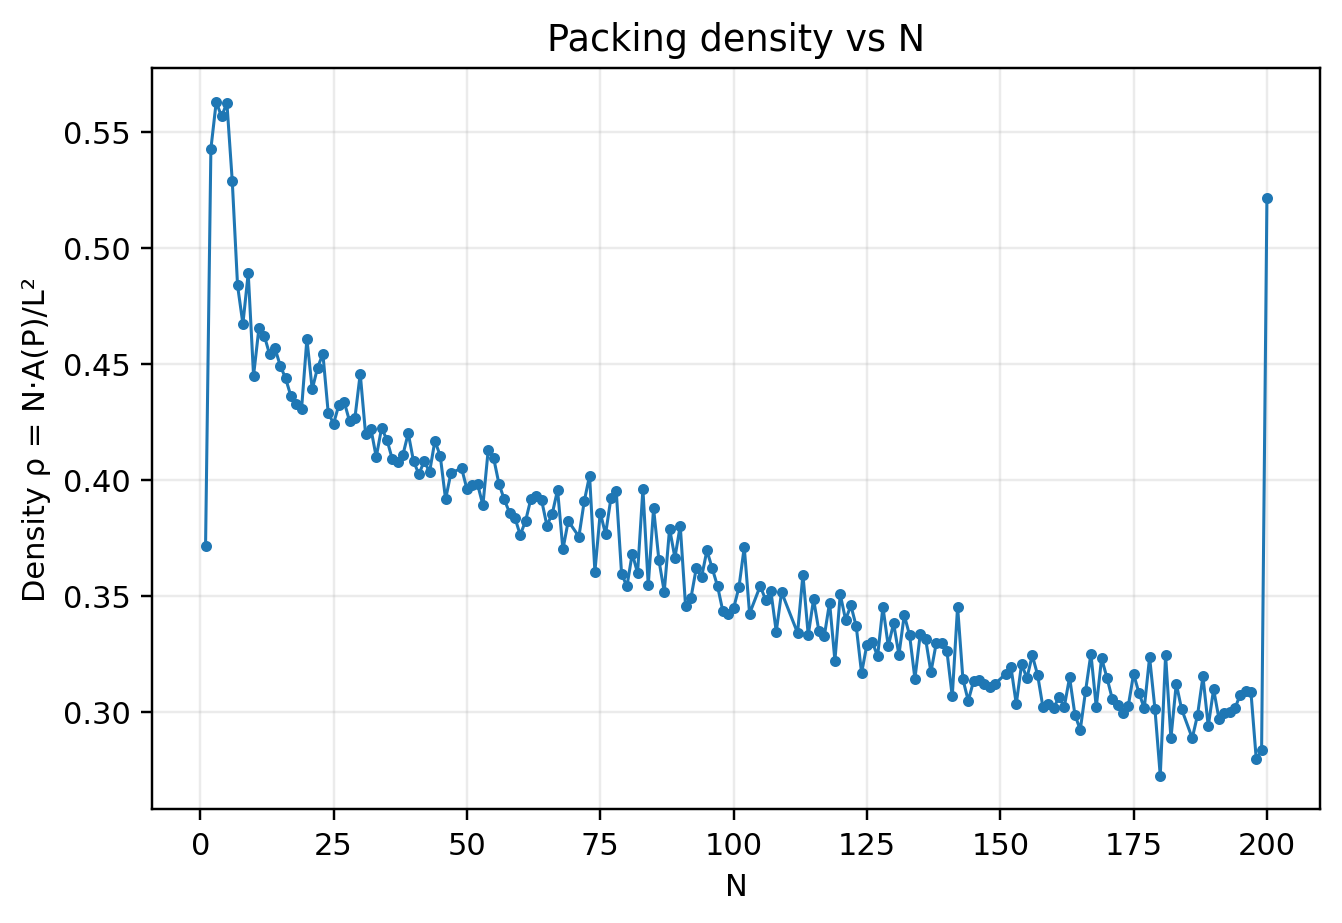
\includegraphics[width=\linewidth]{img/density_vs_N}
    \caption{Best packing efficiency $\eta$ versus $N$. Density
    declines monotonically, driven by both boundary geometry and the
    fixed iteration budget that under-explores larger configuration
    spaces.}
    \label{fig:densityN}
  \end{minipage}
  \hfill
  \begin{minipage}[t]{0.49\linewidth}
    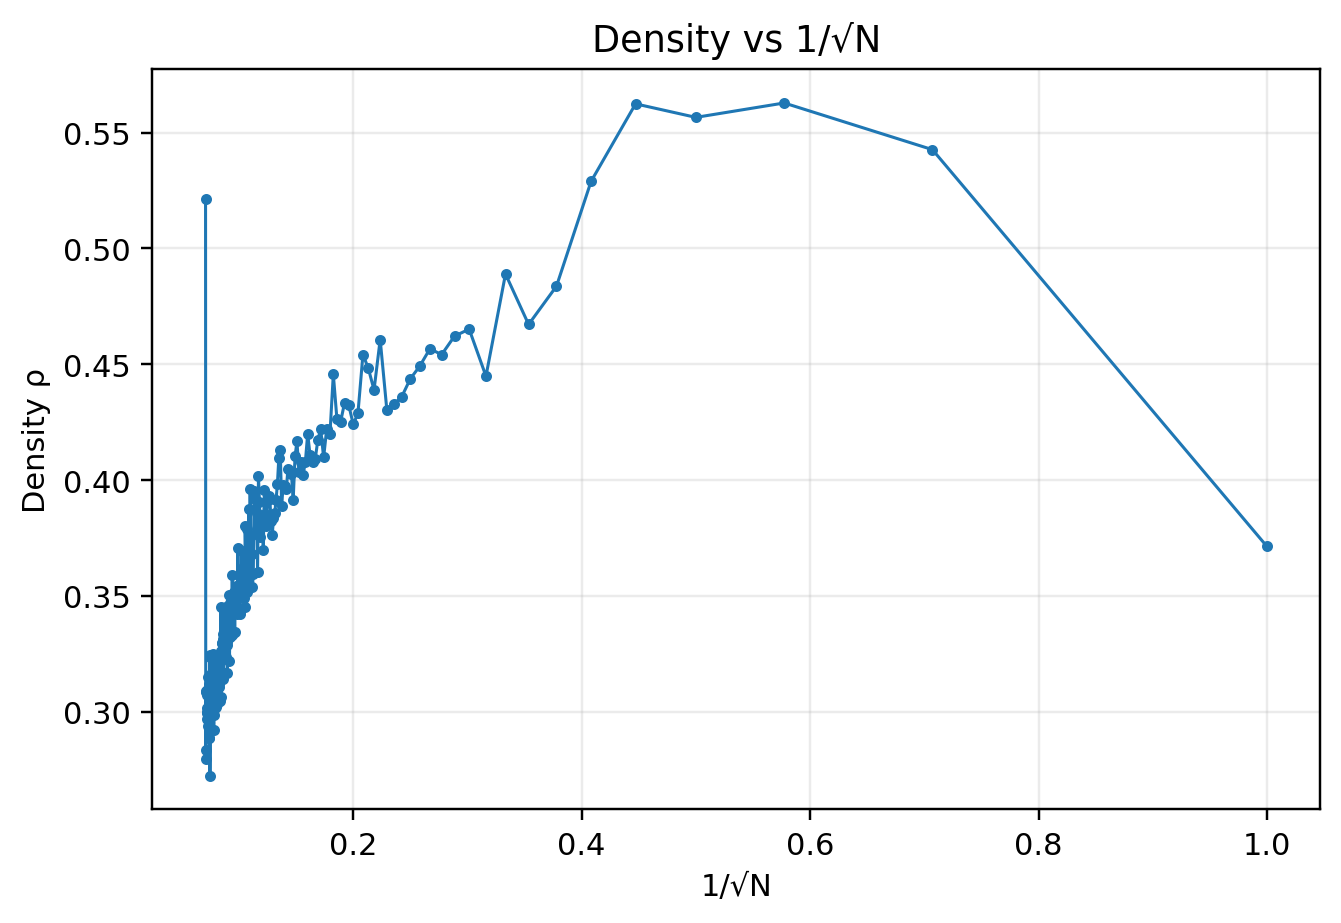
\includegraphics[width=\linewidth]{img/density_vs_inv_sqrtN}
    \caption{Packing efficiency $\eta$ versus $1/\!\sqrt{N}$. The
    approximately linear trend supports $\eta(N) \approx \eta_\infty +
    c/\!\sqrt{N}$ with $\eta_\infty \approx 0.40$, consistent with the
    perimeter-to-area boundary argument.}
    \label{fig:scaling}
  \end{minipage}
\end{figure*}

\end{document}